\section{Resultados}
%###########################
%########## AVG ############
\subsection{Dinámicas factorizables}
\begin{frame}{Dinámicas factorizables}
    Por dinámicas factorizables entendemos\pause:
    \begin{equation}
        \mcH=\sum_{k=1}^{n}\omega_{k}\Id_{2^{k-1}}\otimes H_{k} \otimes \Id_{2^{n-k}},\nonumber
    \end{equation}
    Las unitarias:\pause
    \begin{equation}
        \mcU_{t}=\Motimes_{k=1}^{n}\text{exp}\qty(-\rmi\omega_{k}H_{k}t)=\Motimes_{k=1}^{n} U_{k}(t).\nonumber
    \end{equation}\pause
    \begin{columns}
        \begin{column}{0.5\textwidth}
            El estado de máxima entropía es\pause
            \begin{equation}
                \varrho_{\max}(t)=\Motimes_{k=1}^{n}U_{k}(t) {\color{blue}\qty(\frac{e^{\qty(p_{k}\sum_{j}\lambda_{j}\pauli{j})}}{Z})} (U_{k}(t))^{\dag}\nonumber
            \end{equation}
        \end{column}
        \pause
        \begin{column}{0.5\textwidth}
            La dinámica efectiva tiene expresión general\pause
            \begin{equation}
                \Gamma_{t}(\rho_{\ef})=\sum_{k=1}^{n}p_{k} U_{k}(t) {\color{blue}\rho_{k}} (U_{k}(t))^{\dag}.\nonumber
            \end{equation}
        \end{column}
    \end{columns}
\end{frame}
\begin{frame}{Partículas no interactuantes con diferente frecuencia de transición}
    \begin{columns}
        \begin{column}{0.5\textwidth}
            Hamiltoniano: $\mcH=\sum_{k=1}^{n}\omega_{k}\pauli{3,k}$.\\ \pause
            Usaremos: $\expval{\pauli{k}(t)}_{\ef}=r_{k,\ef}(t)$\\ \pause
            A notar $\expval{\pauli{3}(t)}_{\ef}=\text{cte}$.\\ \pause
            Según lo anterior:
            \begin{equation}
                \expval{\pauli{j}(t)}_{\ef}=\sum_{k=1}^{n}p_{k}\expval{\pauli{j}(t)}_{k}\nonumber
            \end{equation}\pause
            Sea $p_{j\neq 1}=p_{\text{np}}=\frac{1-p_{1}}{1-n}$. Entonces:\pause
            \begin{equation}
                r_{j,\ef}(t)=p_{1}r_{j,1}(t)-\pause p_{\text{np}}r_{\text{np}}\sum_{k=2}^{n}\sin(2\omega_{k} t-\phi_{j})\nonumber
        \end{equation}
        \end{column}
        \pause
        \begin{column}{0.5\textwidth}
            \begin{figure}
                \centering
                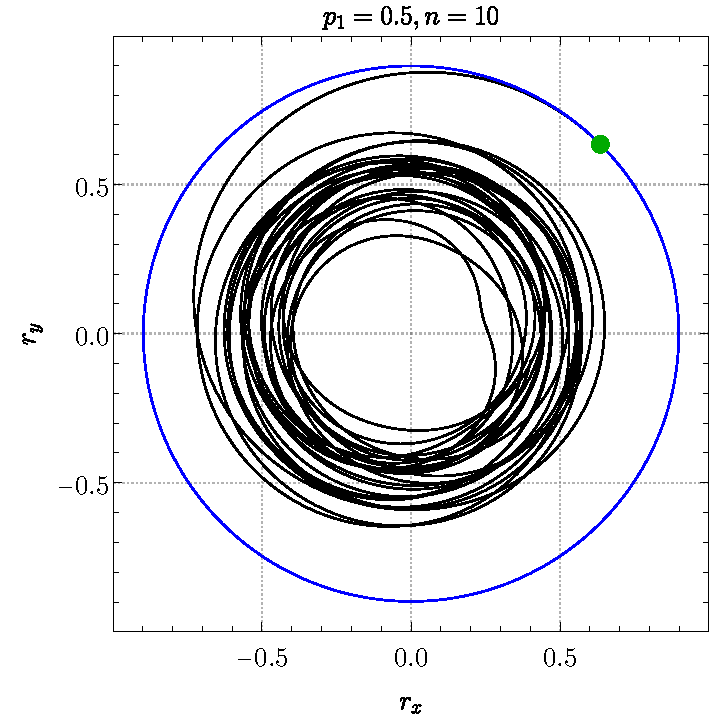
\includegraphics[width=1.\textwidth]{figures/maxent_results/local_all_ran_p=0.5_r=0.9_n=10_a=-3_b=3.pdf}
               \end{figure}
        \end{column}
    \end{columns}
\end{frame}
\begin{frame}{Convergencia}
    \begin{columns}
        \begin{column}{0.5\textwidth}
            Importante: límite $n\rightarrow\infty$. \pause
            \begin{equation}
                \begin{gathered}
                r_{1,\ef}(t)=p_{1}r_{1,1}(t)-p_{\text{np}}r_{\text{np}}{\color{blue}\sum_{k=2}^{n}\sin(2\omega_{k} t-\phi)}\pause\\
                {\color{blue}\sum_{k=2}^{n}\sin(2\omega_{k} t-\phi)}\xrightarrow{n\rightarrow\infty} N(0,\text{std})
                \end{gathered}\nonumber
            \end{equation}\pause
            Pasado algún $t_{\text{s}}$, la dinámica efectiva tiende a\\ \pause
            $\Gamma_{t>t_{\text{s}}}(\vec{r}_{\ef})\xrightarrow{n\rightarrow\infty}\begin{pmatrix}
                p_{1}r_{1,1}(t)\\
                p_{1}r_{2,1}(t)\\
                r_{3}\\
            \end{pmatrix}$\\ \pause
            La dinámica \textbf{converge}.
        \end{column}
        \pause
        \begin{column}{0.5\textwidth}
           \begin{figure}
            \centering
            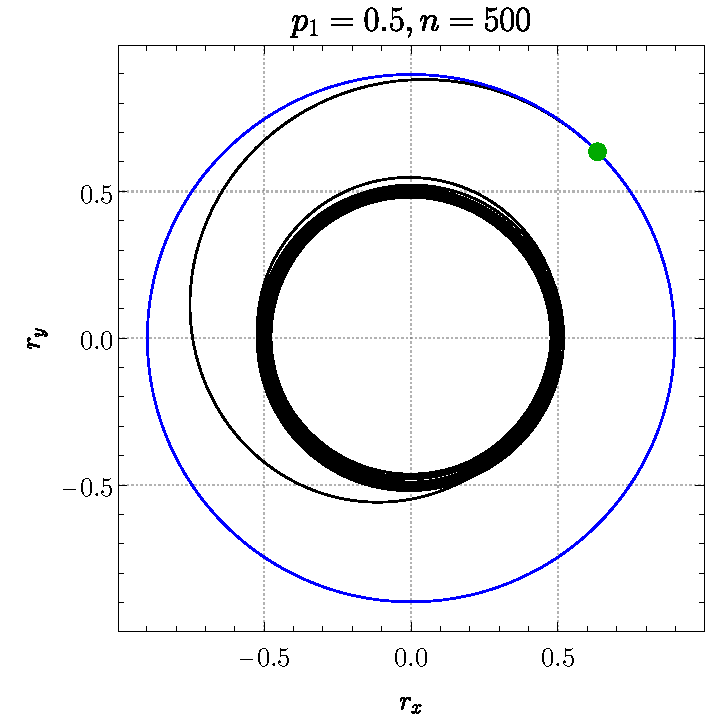
\includegraphics[width=1.\textwidth]{figures/maxent_results/local_all_ran_p=0.5_r=0.9_n=500_a=-3_b=3.pdf}
           \end{figure}
        \end{column}
    \end{columns}
\end{frame}
%###########################


%###########################
%########## AVG ############
\subsection{Compuertas de cómputo cuántico}
\begin{frame}{Compuerta SWAP}
    \begin{columns}
        \begin{column}{0.5\textwidth}
            Estado efectivo antes y después:
            \begin{align*}
                \rho_{\ef}(0)&=p\rho_{A}+(1-p)\rho_{B},\\
                \rho_{\ef}(t=1)&=(1-p)\rho_{A}+p\rho_{B}.
                \end{align*}\pause
                Esto es una contracción:
                \begin{equation*}
                    \kappa_{t}=\frac{r_{\rho_{\ef}(1)}}{r_{\rho_{\ef}(0)}}.
                  \end{equation*}\pause
                  Canal de despolarización \textbf{no lineal}:\pause
                  \begin{center}
                    \tcbox{$\rho_{\ef}\mapsto\kappa_{1}^{\rho_{\ef}}\rho_{\ef}+(1-\kappa_{1}^{\rho_{\ef}})\frac{1}{2}\Id$}
                  \end{center}
        \end{column}\pause
        \begin{column}{0.5\textwidth}
            \begin{figure}[h!]
                \centering
                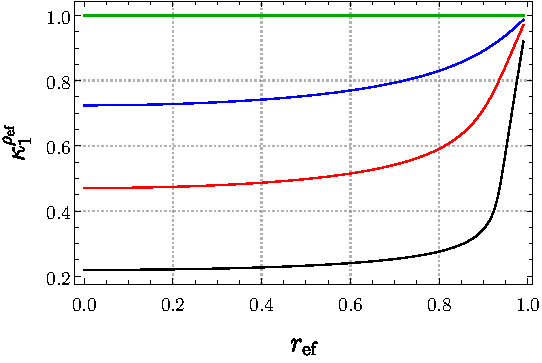
\includegraphics[width=0.9\linewidth]{figures/maxent_results/K(r).pdf}
                \caption{Coeficiente de despolarización como function de $r_{\rho_{\ef}(0)}$ para diferentes valores de $p$.}
              \end{figure}
        \end{column}
    \end{columns}
\end{frame}
\begin{frame}{Compuerta CNOT}
    \begin{columns}
        \begin{column}{0.5\textwidth}
            Estudiamos:
            \begin{equation}
                \rho_{\ef}(t=1)=\CG{\cnot \mcA_{\mcC}^{max}[\rho_{\ef}(0)](\cnot)^{\dag}}\nonumber
            \end{equation}
        \end{column}\pause
        \begin{column}{0.5\textwidth}
            El estado efectivo inicial es
            \begin{equation}
                \rho_{\ef}(0)=p\rho_{A}+(1-p)\rho_{B}.\nonumber
            \end{equation}
        \end{column}\pause
    \end{columns}
    El estado efectivo final es\pause
    \begin{align*}
        \rho_{\ef}(t=1)=&\frac{1}{2}\rho_{\ef}(0)\\
        &+\frac{(1-p)}{2}\qty[{\color{red}\expval{\pauli{1}}_{\rho_{B}}\rho_{A}+(1-\expval{\pauli{1}}_{\rho_{B}})\pauli{3}\rho_{A}\pauli{3}}]\\
        &+\frac{p}{2}\qty[{\color{blue}\expval{\pauli{3}}_{\rho_{A}}\rho_{B}+(1-\expval{\pauli{3}}_{\rho_{A}})\pauli{1}\rho_{B}\pauli{1}}].
    \end{align*}\pause
    \tcbox{Combinación de un canal \textbf{no lineal} de {\color{red}desfasamiento} y un canal \textbf{no lineal} de {\color{blue}bit flip}.}
\end{frame}
%###########################


%###########################
%########## AVG ############
\subsection{Dinámicas especiales}

\begin{frame}{Canales de Pauli}
    \begin{columns}
        \begin{column}{0.5\textwidth}
            \begin{block}{Sobre un qubit}
            Un canal de Pauli sobre un qubit,
            \begin{equation}
                \begin{gathered}
                P:\densityspace{2} \rightarrow \densityspace{2}\nonumber\pause\\
                P(\rho)=\sum_{k}q_{k}\pauli{k}\rho\pauli{k} \rlap{,}
                \end{gathered}
            \end{equation}\pause
            aplica $\pauli{k}$ con probabilidad $q_{k}$.
        \end{block}
        \end{column}
        \pause
        \begin{column}{0.5\textwidth}
            \begin{block}{Sobre $n$ qubits}
            Un canal de Pauli sobre $n$ qubits:
            \begin{equation}
                \begin{gathered}
                P:\densityspace{2^{n}} \rightarrow \densityspace{2^{n}}\nonumber\pause\\
                P(\varrho)=\sum_{\vec{\alpha}}q_{\vec{\alpha}}\pauli{\vec{\alpha}}\varrho\pauli{\vec{\alpha}},\pause \,\text{ }\, \alpha_{k}\in\{0,1,2,3\} \rlap{.}
                \end{gathered}
            \end{equation}\pause
            donde  $\pauli{\vec{\alpha}}=\pauli{\alpha_{1}}\otimes\pauli{\alpha_{2}}\otimes...\otimes \pauli{\alpha_{n}}$.
        \end{block}
        \end{column}
    \end{columns}
\end{frame}

\begin{frame}{Canales de desfasamiento y despolarización}
    \begin{columns}
        \begin{column}{0.5\textwidth}
            \begin{block}{Desfasamiento}
                \begin{equation}
                    P_{n,\pauli{j}}(\varrho)=\sum_{\vec{\alpha}}q_{\vec{\alpha}}\pauli{\vec{\alpha}}\varrho\pauli{\vec{\alpha}}, \,\text{ }\, \alpha_{k}\in\{0,j\}\nonumber
                \end{equation}\pause
                es  de desfasamiento si $q_{\vec{\alpha}\neq\vec{0}}=\frac{1-q_{\vec{0} }}{2^{n}-1}$. \pause La dinámica efectiva: 
                \begin{equation}
                    \Gamma_{t}(\rho_{\ef})=p_{q_{\vec{0}},n}\rho_{\ef}+(1-p_{q_{\vec{0}},n})\pauli{j}\rho_{\ef}\pauli{j}.\nonumber
                \end{equation}
                ¡Otro canal de desfasamiento!
            \end{block}
        \end{column}\pause
        \begin{column}{0.5\textwidth}
            \begin{block}{Despolarización}
                \vspace{0.3cm}
                \begin{equation}
                    D_{q}(\varrho)=q\varrho+(1-q)\frac{\Id_{2^{n}}}{2^n}\nonumber
            \end{equation}\pause
            \vspace{0.3cm}
            
                La dinámica efectiva que corresponde al canal de despolarización es\pause
                \begin{equation}
                    \Gamma_{t}(\rho_{\ef})=q\rho_{\ef}+(1-q)\frac{\Id_{2}}{2},\nonumber
                \end{equation}\pause
                ¡Otro canal de despolarización!
            \end{block}
        \end{column}
    \end{columns}
\end{frame}

\begin{frame}{Canal de estabilización}
    \begin{columns}
        \begin{column}{0.5\textwidth}
            El canal de estabilización.
            \begin{equation}
                \mcE_{\psi,t}(\varrho)=e^{-t\mu}\varrho+(1-e^{-t \mu})\dyad{\psi}\rlap{.}\nonumber\pause
            \end{equation}
            donde $\dyad{\psi}\in \densityspace{2^{n}}$
        \end{column}\pause
        \begin{column}{0.5\textwidth}
            La dinámica efectiva:\pause
            \begin{equation}\label{eq:EffectiveStabilizing}
                \Gamma_{t}(\rho_{\ef})=e^{-t\mu}\rho_{\ef}(0)+(1-e^{-t \mu})\mcC(\dyad{\psi}).\nonumber
            \end{equation}\pause
            ¡Otro canal de estabilización!
        \end{column}
    \end{columns}
\end{frame}
%###########################


%###########################
%########## AVG ############
\subsection{La asignación promedio}
\begin{frame}{Construcción de la asignación promedio}
    Otra forma de escoger un estado microscópico compatible \pause es tomando un promedio\mycite{Macro-To-Micro}. \pause Un promedio sobre el conjunto \pause
    \begin{equation}
        \Omega_{\mcC}(\rho_{\ef}) = \{\ket{\psi}\in\hilbert_{2^{n}}:\, \mcC(\dyad{\psi}) = \rho_{\ef}  \}.\nonumber
    \end{equation}\pause
    La aplicación de asignación promedio\mycite{priv}: \pause
    \begin{equation}
        \mcA_{\mcC}^{\avg}(\rho_{\ef}) =\int d \mu\,\, \delta(\mcC(\dyad{\psi})-\rho_{\ef})\,\dyad{\psi}.\nonumber
    \end{equation} \pause
    ¿Difiere la dinámica observable para diferentes asignaciones?
\end{frame}
\begin{frame}{Distancia entre la asignación promedio y la de máxima entropía}
    \begin{columns}
        \begin{column}{0.5\textwidth}
            \begin{figure}
                \centering
                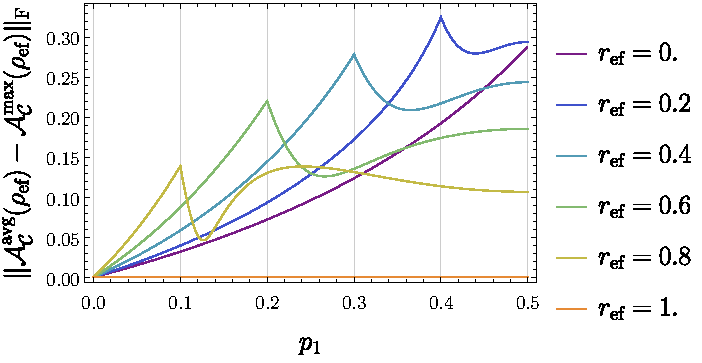
\includegraphics[width=1.\linewidth]{figures/avg_results/dist_maxent_avg_vs_p.pdf}
                \caption{Distancia de Frobenius entre asignaciones como función de $p_{1}$ para diferentes valores de $r_{z}$.}
            \end{figure}
        \end{column}
        \pause
        \begin{column}{0.5\textwidth}
            \begin{itemize}
                \item Iguales si $\rho_{ef}$ es puro o si ($p_{1}\in\{0,1\}$).\pause
                \item Notar que $\mcA_{\mcC}^{\max}(\Id_{2}/2)=\Id_{4}/4$ mientras que $\mcA_{\mcC}^{\avg}(\Id_{2}/2)\neq\Id_{4}/4$.\pause
                \item $\mcA_{\mcC}^{\max}$ puede ser modificado para hacer las mismas suposiciones que $\mcA_{\mcC}^{\avg}$.\pause
            \end{itemize}
        \end{column}
    \end{columns}
    \tcbox{La dinámica efectiva es dependiente de la aplicación de asignación que se utilice}
\end{frame}

%###########################
